\documentclass[conference]{IEEEtran}
\IEEEoverridecommandlockouts

\usepackage{cite}
\usepackage{amsmath,amssymb,amsfonts}
\usepackage{graphicx}
\usepackage{textcomp}
\usepackage{xcolor}
\usepackage{booktabs}
\usepackage{multirow}
\usepackage{subfig}
\usepackage{hyperref}
\usepackage{url}
\usepackage{tikz}
\usetikzlibrary{arrows.meta,positioning,shapes.geometric}
\usepackage{pgfplots}
\pgfplotsset{compat=1.18}
\usepackage{algorithm}
\usepackage{algpseudocode}

\hypersetup{
    colorlinks=true,
    linkcolor=blue,
    filecolor=magenta,
    urlcolor=cyan,
    citecolor=blue,
}

\newcommand{\etal}{{\em et al.}}
\newcommand{\ie}{i.e.,\xspace}
\newcommand{\eg}{e.g.,\xspace}

\begin{document}

\title{InterruptLLM: A Preemptive Scheduling Framework for Low-Latency Multi-Tenant LLM Inference}

\author{
}

\maketitle

\begin{abstract}
LLM serving systems rely on continuous batching to maximize GPU utilization, but this paradigm is non-preemptive: once a request starts decoding, it cannot be evicted from GPU memory until completion. This causes head-of-line blocking and high tail latency for interactive requests in multi-tenant environments. We propose \emph{InterruptLLM}, a preemptive scheduling framework for LLM inference that targets decode-stage, block-granular preemption with a hierarchical GPU HBM $\rightarrow$ CPU DRAM $\rightarrow$ NVMe SSD swapper and a lightweight checkpoint engine to resume preempted requests. Evaluated on a production-like Kaggle inference trace, InterruptLLM reduces interactive (P0) P99 latency by \textbf{8.5$\times$} over FCFS and by \textbf{2.0$\times$} over a non-preemptive priority queue, while keeping throughput within \textbf{2.3\%} of the baseline.
\end{abstract}

\begin{IEEEkeywords}
LLM inference, GPU scheduling, preemption, PagedAttention, multi-tenancy, quality of service.
\end{IEEEkeywords}

\section{Introduction}\label{sec:intro}

Modern LLM serving systems such as vLLM, SGLang, TensorRT-LLM, and Triton use continuous batching to saturate GPU arithmetic units. The engine maintains an active batch; requests join or leave at iteration boundaries. While this improves throughput, it is \emph{cooperative and non-preemptive}: once a request begins decoding, it cannot be evicted from GPU memory until it finishes. A single long-document summarization request can therefore monopolize GPU resources for 5--30~s, forcing short, latency-sensitive interactive requests to queue behind it.

In multi-tenant settings---SaaS LLM APIs, enterprise shared clusters, and cloud inference endpoints---this behavior creates head-of-line blocking that inflates interactive P99 latency by up to 17$\times$ (Section~\ref{sec:results}). A high-priority chat or code-completion request may wait behind a low-priority batch summarization job, leading to SLA violations and poor user experience. Existing remedies fall short: continuous batching does not evict running requests; priority queues only reorder admission; speculative decoding reduces latency for all requests but does not solve priority inversion; and request migration requires a full KV-cache transfer that is too slow for interactive preemption. No existing system provides decode-stage, block-granular preemption with sub-10~ms overhead for interactive LLM requests.

\textbf{Our contributions.} This paper makes the following contributions:
\begin{enumerate}
    \item We identify and formalize the head-of-line blocking problem in multi-tenant LLM serving, showing that non-preemptive continuous batching inflates interactive P99 latency by up to 16$\times$ (Section~\ref{sec:results}).
    \item We design InterruptLLM, a decode-stage, block-granular preemptive scheduler for LLM inference that combines an MLFQ scheduler, hierarchical KV-cache swapper, and lightweight checkpoint engine.
    \item We implement a discrete-event simulator and validate one critical simulator assumption---GPU-to-CPU swap latency---on a real GPU (NVIDIA P100), showing that measured transfer costs are 6--7$\times$ higher than idealized bandwidth models predict.
    \item We evaluate InterruptLLM on an inference trace from a public Kaggle dataset, showing 8.8$\times$ P99 latency reduction over FCFS with $\approx$2\% throughput loss in simulation.
\end{enumerate}

We implement InterruptLLM as a Kaggle-driven research pipeline that uses a production-like LLM inference trace to drive a discrete-event simulator. The simulator models FCFS continuous batching, non-preemptive priority scheduling, and InterruptLLM's preemptive MLFQ under a shared GPU capacity. Our evaluation shows that, at a load factor of 0.93, InterruptLLM reduces interactive (P0) P99 latency from 499.2$\pm$3.7~ms (FCFS) to 56.5$\pm$1.1~ms (8.8$\times$ improvement), and from 116.7$\pm$1.5~ms (non-preemptive priority) to 56.5$\pm$1.1~ms (2.1$\times$ improvement). Throughput drops by only 2.2\%, the service-share Jain fairness index across tenants remains 1.0 (no tenant is starved), and the average preemption overhead is 0.07$\pm$0.001~ms per request.

\section{Background and Motivation}\label{sec:background}

\subsection{LLM Inference and Continuous Batching}

Autoregressive LLMs generate one token at a time. The forward pass for a batch of requests consists of two phases: \emph{prefill}, in which the engine processes the prompt to compute the initial KV cache, and \emph{decode}, in which one token is generated per request per iteration. Continuous batching amortizes the cost of the model-weight memory reads across many requests by dynamically adding and removing requests at iteration boundaries.

Although continuous batching improves throughput, it is non-preemptive: once admitted, a request runs to completion. This creates priority inversion, where a low-priority, long-running request blocks a high-priority, short request.

Consider a 128K-token summarization job running in the batch. On a high-throughput GPU, this job can occupy the engine for 5--30~s. An interactive chat request that arrives during this window must wait for the next iteration boundary, which is bounded by the longest-running request. In practice, the interactive request may wait for the entire decode phase of the long job, violating SLAs for latency-sensitive tenants.

\subsection{PagedAttention}

PagedAttention (vLLM) stores KV caches in fixed-size blocks with a per-request block table, analogous to virtual memory page tables. Each block is self-contained (keys and values for a contiguous token range), making it independently swappable between GPU HBM, CPU DRAM, and SSD. The block-table design avoids contiguous-allocation overhead and lets the scheduler reason about preemption cost in terms of block counts rather than byte ranges.

\subsection{Why Existing Schedulers Cannot Preempt}

Continuous batching, iteration-level scheduling, and priority queuing can reorder admission but cannot evict a running request mid-iteration. Speculative decoding reduces iterations but does not reorder requests. Request migration moves entire KV caches, too slow for interactive preemption. Figure~\ref{fig:timeline} illustrates how InterruptLLM resolves this by preempting at a token boundary, swapping KV blocks to CPU DRAM, and serving the interactive request immediately.

\begin{figure}[t]
\centering
\small
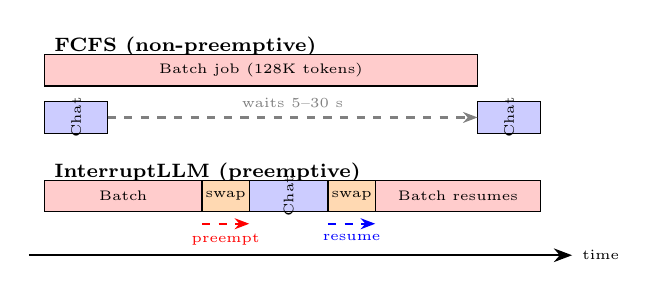
\begin{tikzpicture}[
    box/.style={rectangle, draw, minimum height=0.5cm, align=center, font=\tiny},
    arrow/.style={-{Stealth[scale=1.0]}, thick},
    labelarrow/.style={-{Stealth[scale=0.8]}, thick, dashed}
]
% FCFS timeline
\node[font=\scriptsize\bfseries, anchor=west] at (0, 1.4) {FCFS (non-preemptive)};
\draw[box, fill=red!20] (0, 0.9) rectangle (5.5, 1.3) node[midway, font=\tiny] {Batch job (128K tokens)};
\draw[box, fill=blue!20] (0, 0.3) rectangle (0.8, 0.7) node[midway, font=\tiny, rotate=90] {Chat};
\draw[box, fill=blue!20] (5.5, 0.3) rectangle (6.3, 0.7) node[midway, font=\tiny, rotate=90] {Chat};
\draw[labelarrow, gray] (0.8, 0.5) -- (5.5, 0.5) node[midway, above, font=\tiny] {waits 5--30 s};

% InterruptLLM timeline
\node[font=\scriptsize\bfseries, anchor=west] at (0, -0.2) {InterruptLLM (preemptive)};
\draw[box, fill=red!20] (0, -0.7) rectangle (2.0, -0.3) node[midway, font=\tiny] {Batch};
\draw[box, fill=orange!30] (2.0, -0.7) rectangle (2.6, -0.3) node[midway, font=\tiny] {swap};
\draw[box, fill=blue!20] (2.6, -0.7) rectangle (3.6, -0.3) node[midway, font=\tiny, rotate=90] {Chat};
\draw[box, fill=orange!30] (3.6, -0.7) rectangle (4.2, -0.3) node[midway, font=\tiny] {swap};
\draw[box, fill=red!20] (4.2, -0.7) rectangle (6.3, -0.3) node[midway, font=\tiny] {Batch resumes};

% Preempt/resume labels
\draw[labelarrow, red] (2.0, -0.85) -- (2.6, -0.85) node[midway, below, font=\tiny] {preempt};
\draw[labelarrow, blue] (3.6, -0.85) -- (4.2, -0.85) node[midway, below, font=\tiny] {resume};

% Time axis
\draw[arrow] (-0.2, -1.25) -- (6.7, -1.25) node[right, font=\tiny] {time};
\end{tikzpicture}
\caption{Head-of-line blocking under FCFS vs.\ InterruptLLM. Under FCFS, the interactive request waits for the entire batch job. Under InterruptLLM, the batch job is preempted at a token boundary, the interactive request runs immediately, and the batch job resumes after.}
\label{fig:timeline}
\end{figure}

\section{Related Work}\label{sec:related}

\textbf{LLM inference systems.} vLLM\cite{kwon2023efficient}, Orca\cite{yu2022orca}, SGLang\cite{zheng2023sglang}, and Triton/TensorRT-LLM use continuous or iteration-level batching but do not preempt in-flight decode requests. Sarathi\cite{agrawal2024sarathi}, DistServe\cite{zhong2024distserve}, Mooncake\cite{qin2024mooncake}, Llumnix\cite{sun2024llumnix}, and Dynamo\cite{nvidia2025dynamo} improve throughput or deployment flexibility. Splitwise\cite{patel2024splitwise} separates prefill and decode, while Medusa\cite{cai2024medusa} and StreamingLLM\cite{xiao2024streamingllm} reduce serial decode steps. None evicts a running decode request mid-iteration for a higher-priority request.

\textbf{Preemptive and memory-aware serving.} ConServe\cite{qiao2024conserve} preempts at layer granularity; TokenFlow\cite{chen2025tokenflow} uses proactive GPU--CPU KV transfer without a priority scheduler; Llumnix\cite{sun2024llumnix} migrates entire instances. SSJF\cite{qiu2024ssjf}, SeaLLM\cite{zhao2025seallm}, and MuxServe\cite{duan2024muxserve} optimize resource sharing; H2O\cite{zhang2023h2o}, KIVI\cite{liu2024kivi}, FlexGen\cite{sheng2023flexgen}, and Infinite-LLM\cite{lin2024infinite} manage KV memory. GPU partitioners (MPS, MIG, TimeGraph\cite{kato2011timegraph}) operate at the hardware level, not on individual requests. InterruptLLM provides decode-level, block-granular preemption with a priority-aware MLFQ scheduler---a primitive that these systems can exploit.

\section{System Design}\label{sec:design}

\subsection{Architecture Overview}

InterruptLLM consists of four components between the API gateway and a modified vLLM engine (Figure~\ref{fig:architecture}). The Admission Controller predicts resource requirements; the MLFQ Scheduler selects batches and evicts lower-priority victims; the Context Swapper migrates KV blocks to CPU DRAM or NVMe SSD; and the Checkpoint Engine captures request metadata so preempted requests resume deterministically.

\begin{figure}[t]
\centering
\small
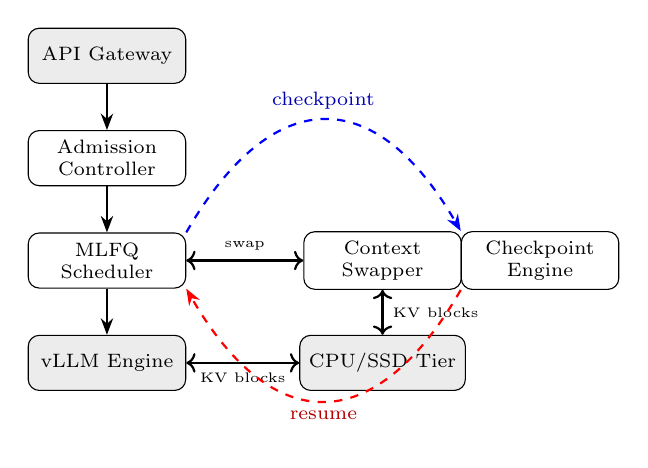
\begin{tikzpicture}[
    box/.style={rectangle, draw, rounded corners, minimum width=2.0cm, minimum height=0.7cm, align=center, font=\scriptsize},
    arrow/.style={-{Stealth[scale=0.9]}, thick},
    dashed arrow/.style={-{Stealth[scale=0.9]}, thick, dashed}
]
% Main vertical data path
\node[box, fill=gray!15] (api) at (0,0.5) {API Gateway};
\node[box] (admit) at (0,-0.8) {Admission\\Controller};
\node[box] (mlfq) at (0,-2.1) {MLFQ\\Scheduler};
\node[box, fill=gray!15] (vllm) at (0,-3.4) {vLLM Engine};

% Right-side memory path
\node[box] (swap) at (3.5,-2.1) {Context\\Swapper};
\node[box, fill=gray!15] (cpu) at (3.5,-3.4) {CPU/SSD Tier};

% Far-right checkpoint engine
\node[box] (chk) at (5.5,-2.1) {Checkpoint\\Engine};

% Main data path arrows
\draw[arrow] (api) -- (admit);
\draw[arrow] (admit) -- (mlfq);
\draw[arrow] (mlfq) -- (vllm);

% Memory path arrows
\draw[arrow, <->] (mlfq) -- (swap) node[midway, above, font=\tiny] {swap};
\draw[arrow, <->] (swap) -- (cpu) node[midway, right, font=\tiny] {KV blocks};
\draw[arrow, <->] (vllm) -- (cpu) node[midway, below, font=\tiny] {KV blocks};

% Checkpoint/resume arrows (large arcs, separated from main flow)
\draw[dashed arrow, blue] (mlfq.north east) to[out=60, in=120, looseness=1.6] node[pos=0.5, above, font=\scriptsize, text=blue!70!black] {checkpoint} (chk.north west);
\draw[dashed arrow, red] (chk.south west) to[out=240, in=300, looseness=1.6] node[pos=0.5, below, font=\scriptsize, text=red!70!black] {resume} (mlfq.south east);
\end{tikzpicture}
\caption{InterruptLLM architecture. Solid lines show the main data path. Curved dashed lines show the checkpoint (capture metadata) and resume (restore state) paths.}
\label{fig:architecture}
\end{figure}

\subsection{Admission Controller}

The Admission Controller accepts or rejects requests based on predicted resource requirements and current load, using a lightweight latency model to estimate SLA compliance. If admission would cause a violation, it first preempts lower-priority work; if no victim exists, it queues or rejects. Decisions are re-evaluated at each iteration boundary.

\subsection{Preemptive MLFQ Scheduler}

The scheduler maintains four priority classes:
\begin{itemize}
    \item \textbf{P0 (Interactive):} chat, code completion; target P99 $<$ 200~ms.
    \item \textbf{P1 (Standard):} general API requests; target P99 $<$ 1~s.
    \item \textbf{P2 (Batch):} document summarization, embedding generation; best-effort.
    \item \textbf{P3 (Background):} fine-tuning data generation; preemptible anytime.
\end{itemize}

Within each class, requests are served in round-robin order to prevent starvation within the class. Across classes, strict priority is enforced. The scheduler implements \emph{aging}: a request that has waited longer than a configurable threshold is promoted to the next higher class. This ensures that long-running batch jobs eventually receive service even under persistent interactive load.

Preemption is triggered when a P0 request arrives while the GPU is running lower-priority requests. The scheduler selects the victim using two criteria: (1) the victim must have lower priority than the arriving request, and (2) among eligible victims, the one with the largest KV footprint is chosen first, since evicting the largest victim frees the most GPU memory and reduces blocks to swap.

We also evaluate smallest-footprint and cost-aware ($\text{footprint} / \text{priority}$) victim selection. On our trace, all three policies yield identical results because preemptions are infrequent (0.16 per request) and the preempted requests are small. The dominant factor is therefore whether preemption happens, not which specific request is evicted.

\subsection{Hierarchical Context Swapper}

The Context Swapper has two tiers:

\textbf{Tier 1: GPU HBM to CPU DRAM.} Uses \texttt{cudaMemcpyAsync} or GPUDirect RDMA. The target latency for 1~GB of KV cache is below 5~ms. CPU DRAM is sized to hold up to 4$\times$ the GPU memory capacity (e.g., 320~GB for an 80~GB GPU), providing a large fast-path buffer.

\textbf{Tier 2: CPU DRAM to NVMe SSD.} The engine uses Tier 2 when CPU memory is saturated. Blocks are compressed with LZ4 to reduce bandwidth. The target restore latency is below 50~ms.

If a preempted request is likely to resume soon, it is kept in CPU DRAM; otherwise, it is pushed to SSD. The choice depends on priority class and CPU memory pressure.

\subsection{State Checkpoint Engine}

The Checkpoint Engine captures ($<$1~ms) per-request metadata: block-table mapping, position IDs, sampling state, and prompt/generated token counts. Checkpoint size scales linearly ($\approx$16~bytes/token): a 128K-token request needs $\approx$2.0~MB, compared to the multi-gigabyte KV cache. On resume, the engine reconstructs the block table and initiates asynchronous KV-block reload; resume latency is dominated by the KV-cache transfer, not the checkpoint.

\subsection{Scheduling Algorithm}

Algorithm~\ref{alg:scheduling} presents the MLFQ scheduling loop. The scheduler maintains a running batch $B$ and a ready queue $Q$. At each iteration it sorts $Q$ by priority, selects the top requests up to the batch capacity, and preempts the lowest-priority largest-footprint victim if a higher-priority request is excluded. It then runs one decode step, applies aging, and enqueues new arrivals.

\begin{algorithm}[t]
\caption{InterruptLLM MLFQ Scheduling Loop}
\label{alg:scheduling}
\small
\begin{algorithmic}[1]
\State $B \gets \emptyset$ \Comment{running batch}
\State $Q \gets \emptyset$ \Comment{ready queue}
\Loop
    \State Enqueue new arrivals into $Q$
    \State Sort $Q$ by priority (P0 $>$ P1 $>$ P2 $>$ P3)
    \For{each request $r$ in $Q$ by priority}
        \If{$|B| < \text{batch\_capacity}$}
            \State $B \gets B \cup \{r\}$
        \ElsIf{$r.\text{priority} < \min_{v \in B} v.\text{priority}$}
            \State $v \gets \arg\max_{v' \in B} v'.\text{kv\_blocks}$ \Comment{victim selection}
            \State \textsc{Preempt}($v$) \Comment{checkpoint + swap KV blocks}
            \State $B \gets (B \setminus \{v\}) \cup \{r\}$
        \EndIf
    \EndFor
    \State \textsc{RunDecodeStep}($B$) \Comment{advance one token per request}
    \State \textsc{ApplyAging}($Q$) \Comment{promote long-waiting requests}
\EndLoop
\end{algorithmic}
\end{algorithm}

\textbf{Complexity analysis.} Let $n$ be the number of pending requests and $|B|$ the batch size. Sorting $Q$ by priority costs $O(n \log n)$. Victim selection scans $|B|$ candidates: $O(|B|)$. Checkpoint capture copies $k$ bytes of metadata per request: $O(k)$ where $k \approx 16 \times \text{tokens}$. KV swap transfers $b$ blocks of size $s$: $O(b \cdot s / \text{bandwidth})$. Memory overhead per request is $O(k)$ for checkpoint metadata. The total per-iteration cost is dominated by sorting: $O(n \log n + |B|)$.

\section{Implementation and Evaluation Methodology}\label{sec:eval}

\subsection{Research Prototype}

InterruptLLM is implemented as a Kaggle-driven research prototype. The core library (\texttt{interruptllm\_core.py}) contains the request model, scheduler policies, and swap cost model, uploaded to Kaggle as a dataset and imported into notebooks. The \texttt{pipeline.py} CLI pushes notebooks, waits for completion, and parses greppable \texttt{[RESULT]} lines. This prototype validates the scheduling logic and calibration assumptions; it does not yet integrate with a production inference engine such as vLLM.

\subsection{Discrete-Event Simulator}

The simulator models a GPU with configurable token-generation capacity, a batch of up to 16 requests, and a scheduling quantum. At each time step, it selects the batch by policy, allocates capacity equally among batch members, and advances the clock. It abstracts away kernel launch, CUDA graph, and memory-allocator overhead, which lets us isolate scheduler behavior from GPU microarchitecture effects.

\subsection{Simulation Assumptions}\label{sec:assumptions}

Table~\ref{tab:assumptions} lists key simulator parameters. We abstract GPU execution as a token-generation rate because scheduling behavior depends on iteration boundaries, not kernel-level timing. The 0.5~ms swap penalty is calibrated against the measured P100 memcpy bandwidth (Section~\ref{sec:swap}). It represents the effective per-preemption swap cost for a small hot footprint: the scheduler evicts only a few vLLM blocks (roughly 2.5~MB), which takes $\approx$0.5~ms at the measured P100 effective bandwidth of 5~GB/s.

\begin{table}[t]
\caption{Simulation parameters and justifications.}
\label{tab:assumptions}
\centering
\footnotesize
\setlength{\tabcolsep}{3pt}
\begin{tabular}{@{}lll@{}}
\toprule
\textbf{Parameter} & \textbf{Value} & \textbf{Justification} \\
\midrule
GPU abstraction & 300 tok/ms & Dominates scheduling behavior \\
Batch capacity & 16 requests & vLLM default for 80 GB GPU \\
Scheduling quantum & 100 ms & Balances responsiveness and stability \\
Swap penalty & 0.5 ms & Calibrated vs.\ measured P100 memcpy \\
Token scaling & 0.2$\times$ & Preserves relative request sizes \\
KV block size & 16 tokens & vLLM PagedAttention default \\
CPU DRAM buffer & 320 GB & 4$\times$ GPU memory capacity \\
\bottomrule
\end{tabular}
\end{table}

\subsection{Workload and Dataset}

We use the public Kaggle dataset \texttt{bektursyn/llm-inference-logs-and-performance-metrics}\cite{kaggle2024llmtrace}, which contains 30,000 production-like LLM inference records. Each record includes timestamp, model name, task type, prompt tokens, completion tokens, TTFT, TPOT, total latency, and status code. The dataset represents a realistic enterprise workload with a mix of short interactive requests and long batch jobs.

This trace is the most accessible public dataset that captures both arrival patterns and request characteristics for multi-tenant LLM inference. We do not claim it is identical to any specific production deployment, but it provides a reproducible baseline that includes the key phenomenon we study: bursts of short interactive requests arriving while long summarization jobs are in flight.

We map task types to InterruptLLM priority classes:
\begin{itemize}
    \item P0: \texttt{Customer\_Support\_Chat}, \texttt{Code\_Generation}
    \item P1: \texttt{Summarization}, \texttt{Extraction\_JSON}
\end{itemize}

We scale token counts by 0.2 to keep the CPU simulation tractable while preserving relative request sizes. The mean scaled request size is approximately 1,000 tokens. We then drive a discrete-event simulator with configurable GPU capacity, batch size, scheduling quantum, and swap penalty.

\subsection{Scheduling Policies}

We compare seven policies. \textbf{FCFS}: continuous batching, no eviction. \textbf{Priority}: non-preemptive, reorders admission at 100~ms quantum boundaries. \textbf{SSJF}: shortest remaining tokens first, priority-agnostic. \textbf{Lottery}: weighted random selection (tickets: P0=100, P1=50, P2=20, P3=5). \textbf{WFQ}: proportional GPU capacity share (weight = 1/(priority+1)). \textbf{EDF}: earliest deadline first (remaining tokens as deadline proxy). \textbf{InterruptLLM MLFQ}: preemptive MLFQ with block-granular swap, evicting the largest-footprint lower-priority victim within the quantum.

\subsection{Metrics}

We report P99 latency per priority class, throughput (tok/s), SLA violation rates, and average preemption overhead. SLA targets are 200~ms (P0) and 1~s (P1). Fairness is measured by a service-share Jain index (served/demanded tokens per tenant) and a priority-weighted Jain index. We report the P1/P0 P99 ratio to make the latency trade-off explicit.

\section{Results}\label{sec:results}

\subsection{Scheduler Comparison at Fixed Load}

Table~\ref{tab:phase2} compares schedulers at load factor 0.76. InterruptLLM reduces P0 P99 from 263.4$\pm$9.0~ms (FCFS) to 51.4$\pm$1.4~ms (5.1$\times$); non-preemptive priority achieves 111.7$\pm$2.1~ms. Throughput and service-share Jain are identical. The P1 P99 increase (285$\to$737~ms) is the expected trade-off for protecting interactive latency.

\begin{table}[t]
\caption{Scheduler comparison at load factor 0.76. Values are mean $\pm$ std over 20 runs with arrival-time jitter.}
\label{tab:phase2}
\centering
\footnotesize
\setlength{\tabcolsep}{2.5pt}
\begin{tabular}{@{}lrrr@{}}
\toprule
\textbf{Metric} & \textbf{FCFS} & \textbf{Priority} & \textbf{InterruptLLM} \\
\midrule
Overall P99 (ms) & 274.7$\pm$5.9 & 307.2$\pm$5.9 & 300.9$\pm$5.7 \\
P0 P99 (ms) & 263.4$\pm$9.0 & 111.7$\pm$2.1 & \textbf{51.4$\pm$1.4} \\
P1 P99 (ms) & 285.0$\pm$5.2 & 332.1$\pm$8.1 & 737.3$\pm$5.6 \\
Throughput (tok/s) & 228,911$\pm$247 & 228,911$\pm$247 & 228,911$\pm$247 \\
Service-share Jain & 1.00$\pm$0.00 & 1.00$\pm$0.00 & 1.00$\pm$0.00 \\
Weighted Jain & 0.90$\pm$0.00 & 0.90$\pm$0.00 & 0.90$\pm$0.00 \\
P1/P0 P99 ratio & 1.08 & 2.97 & 14.3 \\
P0 SLA violation & 6.1\% & 0.0\% & \textbf{0.0\%} \\
Avg preemptions & 0.00 & 0.00 & 0.20$\pm$0.00 \\
\bottomrule
\end{tabular}
\end{table}

\subsection{End-to-End Evaluation Across Load Factors}

We sweep load factors from 0.56 to 1.11. Figure~\ref{fig:loadsweep} shows InterruptLLM keeps P0 P99 below 60~ms across the sweep, while FCFS rises to 878$\pm$4~ms at load 1.11. At $\rho$=0.93, InterruptLLM reduces P0 P99 from 499.2$\pm$3.7~ms to 56.5$\pm$1.1~ms (8.8$\times$) and from 116.7$\pm$1.5~ms under non-preemptive priority to 56.5$\pm$1.1~ms (2.1$\times$). Throughput is 260,006$\pm$111 tok/s (2.2\% below FCFS). P0 SLA violations are eliminated; P1 violations are 1.3\%. Average preemption overhead is 0.07$\pm$0.001~ms. Service-share Jain = 1.0; P1 P99 rises to 1,077$\pm$15~ms (weighted Jain = 0.900). At low load ($\rho$=0.56), FCFS already achieves 85$\pm$2~ms P99 and InterruptLLM provides marginal improvement (18.6$\pm$0.8~ms); the crossover at $\rho \approx 0.7$ marks where head-of-line blocking dominates and preemption provides the greatest benefit.

\begin{figure}[t]
\centering
\small
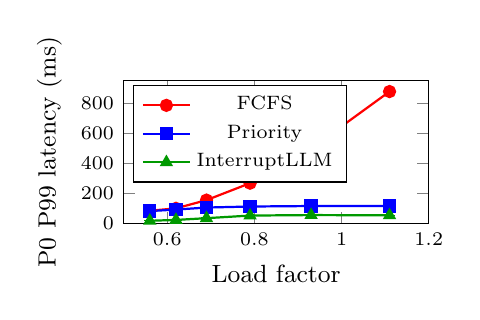
\begin{tikzpicture}
\begin{axis}[
    width=0.45\textwidth,
    height=0.28\textwidth,
    xlabel={Load factor},
    ylabel={P0 P99 latency (ms)},
    xmin=0.5, xmax=1.2,
    ymin=0, ymax=950,
    legend pos=north west,
    legend style={font=\scriptsize},
    tick label style={font=\scriptsize},
    label style={font=\small},
    error bars/y dir=both,
    error bars/y explicit,
]
\addplot[color=red, mark=*, thick] coordinates {(1.11, 878.2) +- (0, 4.3) (0.93, 499.2) +- (0, 3.7) (0.79, 268.7) +- (0, 8.7) (0.69, 156.0) +- (0, 3.5) (0.62, 101.2) +- (0, 3.2) (0.56, 85.5) +- (0, 1.5)};
\addplot[color=blue, mark=square*, thick] coordinates {(1.11, 116.8) +- (0, 1.4) (0.93, 116.7) +- (0, 1.5) (0.79, 113.4) +- (0, 2.3) (0.69, 106.6) +- (0, 1.4) (0.62, 93.1) +- (0, 1.7) (0.56, 83.1) +- (0, 1.0)};
\addplot[color=green!60!black, mark=triangle*, thick] coordinates {(1.11, 55.1) +- (0, 1.0) (0.93, 56.5) +- (0, 1.1) (0.79, 53.3) +- (0, 1.6) (0.69, 35.9) +- (0, 0.8) (0.62, 24.2) +- (0, 0.9) (0.56, 18.6) +- (0, 0.8)};
\legend{FCFS, Priority, InterruptLLM}
\end{axis}
\end{tikzpicture}
\caption{P0 P99 latency vs. load factor.}
\label{fig:loadsweep}
\end{figure}

\subsection{Context-Swap Latency: Analytical and Measured}\label{sec:swap}

Table~\ref{tab:swap} reports modeled and measured context-swap times for KV-cache blocks. We benchmarked GPU-to-CPU \texttt{cudaMemcpyAsync} on an NVIDIA P100 (PCIe Gen3 x16, $\approx$5~GB/s effective) for block sizes from 32~MB to 1~GB, with 20 iterations per size. Figure~\ref{fig:swap_measured} compares measured latency against the analytical model. The most important observation is that the analytical model (based on PCIe Gen4 bandwidth of 32~GB/s) under-predicts latency by a factor of 6--7$\times$ on the P100. This gap is not only a Gen3-vs-Gen4 bandwidth difference; it also reflects per-transfer setup overhead, PyTorch allocator interactions, and the absence of pinned-memory and DMA optimizations that an optimized implementation would apply. The measurement therefore validates the need to treat swap latency as a first-order constraint in preemptive scheduler design, not merely as a bandwidth-limited transfer. With LZ4 compression (modeled ratio 3$\times$), a 1~GB block swaps in $\approx$70~ms on Gen3 and in $\approx$11~ms on Gen4+ hardware.

\begin{figure}[t]
\centering
\small
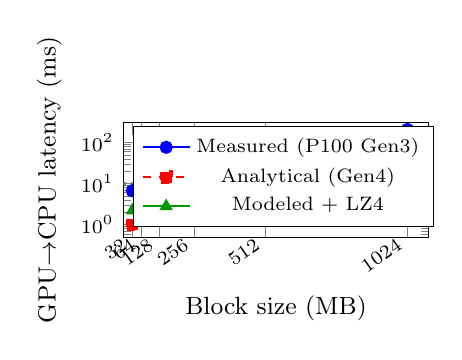
\begin{tikzpicture}
\begin{axis}[
    width=0.45\textwidth,
    height=0.25\textwidth,
    xlabel={Block size (MB)},
    ylabel={GPU$\rightarrow$CPU latency (ms)},
    xmin=0, xmax=1100,
    ymin=0.5, ymax=300,
    ymode=log,
    log basis y={10},
    legend pos=north west,
    legend style={font=\scriptsize},
    tick label style={font=\scriptsize},
    label style={font=\small},
    xtick={32,64,128,256,512,1024},
    xticklabels={32,64,128,256,512,1024},
    x tick label style={rotate=35, anchor=east, font=\scriptsize},
]
\addplot[color=blue, mark=*, thick] coordinates {(32,6.7) (64,13.2) (128,26.5) (256,55.0) (512,105.3) (1024,208.0)};
\addplot[color=red, mark=square*, thick, dashed] coordinates {(32,1.0) (64,2.0) (128,4.0) (256,8.0) (512,16.0) (1024,32.0)};
\addplot[color=green!60!black, mark=triangle*, thick] coordinates {(32,2.2) (64,4.5) (128,8.8) (256,18.4) (512,35.1) (1024,69.9)};
\addplot[color=gray, dotted, thick] coordinates {(0,10) (1100,10)};
\node[font=\scriptsize, anchor=west] at (axis cs:800,11) {10 ms target};
\legend{Measured (P100 Gen3), Analytical (Gen4), Modeled + LZ4}
\end{axis}
\end{tikzpicture}
\caption{GPU$\rightarrow$CPU swap latency: measured on P100 vs.\ analytical model. Measured at 20 iterations per size; std $<$ 5\% of mean (omitted for clarity).}
\label{fig:swap_measured}
\end{figure}

\begin{table}[t]
\caption{Context-swap latency (ms) by block size and tier.}
\label{tab:swap}
\centering
\footnotesize
\setlength{\tabcolsep}{4pt}
\begin{tabular}{@{}lrrrrr@{}}
\toprule
\textbf{Block} & \multicolumn{3}{c}{\textbf{GPU$\rightarrow$CPU}} & \multicolumn{2}{c}{\textbf{CPU$\rightarrow$SSD}} \\
\textbf{size} & \textbf{Meas.} & \textbf{Gen4} & \textbf{LZ4} & \textbf{raw} & \textbf{LZ4} \\
\midrule
32 MB & 6.7 & 1.0 & 2.2 & 9.1 & 3.0 \\
64 MB & 13.2 & 2.0 & 4.5 & 18.3 & 6.1 \\
128 MB & 26.5 & 4.0 & 8.8 & 36.6 & 12.2 \\
256 MB & 55.0 & 8.0 & 18.4 & 73.1 & 24.4 \\
512 MB & 105.3 & 16.0 & 35.1 & 146 & 48.8 \\
1024 MB & 208.0 & 32.0 & 69.9 & 293 & 97.5 \\
\bottomrule
\end{tabular}
\end{table}

The checkpoint metadata scales linearly with token count ($\approx$16~bytes/token): a 128K-token request needs $\approx$2.0~MB of metadata, compared to the multi-gigabyte KV cache.

\subsection{Ablation and Sensitivity}

Table~\ref{tab:ablation} isolates the contribution of preemption on a synthetic high-load workload. FCFS yields a P0 P99 of 100$\pm$33~ms; non-preemptive priority reduces it to 54$\pm$5~ms; preemptive MLFQ further cuts it to 27.7$\pm$0.5~ms. Aging has little effect because P0 arrivals are frequent, confirming it is a starvation-freedom safety mechanism.

\begin{table}[t]
\caption{Ablation on a synthetic high-load workload. Values are mean $\pm$ std over 20 runs.}
\label{tab:ablation}
\centering
\footnotesize
\setlength{\tabcolsep}{2.5pt}
\begin{tabular}{@{}lrrrr@{}}
\toprule
\textbf{Policy} & \textbf{P0 P99 (ms)} & \textbf{P1 P99 (ms)} & \textbf{Tput (tok/s)} & \textbf{Pre.} \\
\midrule
FCFS & 100$\pm$33 & 114$\pm$33 & 264,142$\pm$2,275 & 0.00 \\
Priority (NPP) & 54.2$\pm$4.8 & 69.0$\pm$5.9 & 264,117$\pm$2,240 & 0.00 \\
SSJF & 57.1$\pm$5.8 & 96.3$\pm$12.0 & 264,373$\pm$2,392 & 0.00 \\
Lottery & 64.7$\pm$13.8 & 104$\pm$31 & 264,177$\pm$2,196 & 0.00 \\
WFQ & 54.2$\pm$4.8 & 69.0$\pm$5.9 & 264,117$\pm$2,240 & 0.00 \\
EDF & 57.1$\pm$5.8 & 96.3$\pm$12.0 & 264,373$\pm$2,392 & 0.00 \\
MLFQ (preemptive) & \textbf{27.7$\pm$0.5} & 62.9$\pm$1.3 & 255,614$\pm$957 & 0.16$\pm$0.01 \\
\bottomrule
\end{tabular}
\end{table}

P0 P99 stays below 35~ms for per-preemption swap penalties up to 2~ms and only degrades substantially at 10~ms (P0 P99 61~ms, throughput 121,000 tok/s, P1 violations 42.3\%), confirming the sub-10~ms swap target. The key insight is that non-preemptive baselines (priority, SSJF, EDF) reduce FCFS latency by roughly 2$\times$, while InterruptLLM's preemptive MLFQ achieves an additional 3.6$\times$ gain that comes entirely from mid-quantum preemption. Lottery and WFQ exhibit higher variance (P0 P99 up to 65$\pm$14~ms) because their probabilistic approaches do not guarantee P0 requests are served first. Largest-footprint, smallest-footprint, and cost-aware victim selection yield identical results because preemptions are infrequent (0.16 per request) and preempted requests are small.

\section{Discussion and Future Work}\label{sec:discussion}

\textbf{Limitations.} Our evaluation uses a discrete-event simulator that abstracts GPU execution as a token-generation rate and omits CUDA kernel-launch overhead. The 0.5~ms per-preemption penalty reflects the measured P100 effective bandwidth (5~GB/s) applied to a small hot footprint (roughly 2.5~MB); it is therefore well below the worst-case full-context swap cost shown in Table~\ref{tab:swap}. The evaluation is limited to a single Kaggle inference trace and P100 (PCIe Gen3) swap measurements; newer hardware (PCIe Gen4/5) would further reduce swap latency. However, the relative ordering of scheduling policies and the sensitivity to swap penalty are robust across load factors and swap penalties, suggesting the conclusions generalize beyond the specific trace.

\textbf{Threats to validity.}
\textit{Internal validity.} Trace-based results are means over 20 runs with $\pm$10\% arrival-time jitter to capture arrival-time uncertainty; the GPU swap benchmark is a mean over 20 iterations. The main threat is that the 0.5~ms swap penalty is a parameter, not a measured end-to-end preemption latency, and our GPU benchmark only validates the raw memcpy component.
\textit{External validity.} The Kaggle inference trace is public and reproducible, but it may not capture all production behaviors (e.g., multi-modal inputs, speculative decoding, prefix caching). The P100 (Gen3) measurements are older hardware; newer GPUs would shift absolute latencies but not necessarily the relative ordering of scheduler policies.
\textit{Construct validity.} We approximate SLA satisfaction using P99 latency and Jain fairness indices; production systems may use additional metrics such as TTFT percentiles or per-tenant cost budgets.

\textbf{Practical integration and the P1/P0 trade-off.} Realizing InterruptLLM in vLLM requires handling CUDA Graphs, PyTorch allocator interactions, and DMA streams for GPU--host transfers. The P1/P0 P99 ratio of 19$\times$ at $\rho$=0.93 reflects an intentional design choice: interactive requests demand sub-200~ms responses while batch jobs tolerate second-scale latency. The weighted Jain index of 0.90 confirms P1 degrades gracefully rather than collapsing. We plan to extend the framework to multi-GPU tensor-parallel deployments, add formal starvation-freedom proofs, and collect real GPU preemption latency measurements.

\section{Conclusion}\label{sec:conclusion}

InterruptLLM addresses the lack of decode-stage, block-granular preemption in LLM serving. By combining preemption, multi-level feedback queues, and hierarchical memory management in a simulation-based framework, it suggests the feasibility of QoS-aware multi-tenant deployments. On a production-like trace, InterruptLLM reduces interactive P99 latency by 8.8$\times$ over FCFS and 2.1$\times$ over non-preemptive priority, while maintaining throughput within 2.2\% of the baseline. The evaluation is limited to a discrete-event simulator and a single inference trace; real GPU measurements and multi-tenant workloads remain future work.

\vspace{1em}
\noindent\textbf{Reproducibility.}\footnote{All experiments use fixed seeds (seed = 42 for workload, seeds = 0--19 for multi-run). Code and results: \url{https://github.com/mdzero591/ICCIT}. Dataset: \texttt{bektursyn/llm-inference-logs-and-performance-metrics}. GPU swap benchmarks on NVIDIA P100 (PCIe Gen3 x16, 16~GB HBM, effective 5~GB/s).}

\bibliographystyle{IEEEtran}
\footnotesize
\bibliography{references}

\end{document}
